\documentclass[aps,prl,reprint,groupedaddress]{revtex4-2}
\usepackage{graphicx}    % Required for inserting images.
\usepackage{amsmath,amssymb,gensymb}  % Advanced math formatting.
\usepackage{float}  % Required to force figure position.
\usepackage{lipsum} % For dummy text.
\usepackage{hyperref} % Required to cite links.
\usepackage{siunitx} % Required to typeset units properly.
\usepackage{tikz} % Required for drawing figures.
\usepackage{multirow} % Required for merging table cells.
\usepackage{appendix}

\sisetup{input-digits = 0123456789\pi, uncertainty-mode = separate}%



\begin{document}

\title{Comparing the magnetic field of a current carrying coil to standard electromagnetic models}
\author{Leandro Perez Moran}
\altaffiliation{leandro.perezmoran@gmail.com}
\affiliation{Dawson College, Montreal, Canada}

\begin{abstract}
    \noindent
\textbf{\textit{Abstract:}}
Electromagnetism is a key aspect of our lives. Today, practically all common household items have integrated electrical circuits. A common component in these circuits are electromagnets, whose functions range from the magnetrons in our microwave ovens to the launching systems of aircraft carriers. As such, a thorough understanding of electromagnetism is more important than ever, which is why we set out to compare the measured magnetic field of a current-carrying coil to that predicted by our best model of electromagnetism. Using a Pasco PS-2162 we measured the magnetic field strength along the coil's axis and found all data points to be within \SI{50.4}{\micro\tesla} of the expected values. Additionally, only 3 of the 13 analyzed data points were outside the uncertainty range. Our findings therefore support the validity of our current model of electricity and magnetism.

\begin{center}
    \textbf{Keywords:} \textit{Electricity, magnetism, current carrying coil, magnetic field}
\end{center}
\end{abstract}

\maketitle

\section{Introduction}
The Biot-Savard law, discovered in 1920 by French physicists Jean-Baptiste Biot and Felix Savard, is the fundamental law for understanding magnetism. The law is expressed as follows:

\begin{equation}
    \vec{B}=\frac{\mu_0}{4\pi}\frac{q\vec{v}\times\hat{r}}{r^2}
    \label{eq: Biot-Savard law}
\end{equation}

Where $\mu_o$ is the permeability constant \SI{4\pi e-7}{\tesla\metre\per\ampere}, $\vec{B}$ the magnetic field generated by some particle of charge $q$, $\vec{v}$ the particle's velocity, and $\hat{r}$ and $r$ are respectively a unit vector pointing from the particle to the point where the field is being calculated and the distance between said points. However, this law only applies to point charges. As such, we must adapt it to work with current segments. By definition, current is the rate of change of charge over time, that is 

\begin{equation}
    I\equiv\frac{\text{d} Q}{\text{d}t}
    \label{eq: Current definition}
\end{equation}

Furthermore, in any given section of wire $\Delta\vec{s}$, the velocity of the moving charges is parallel to the segment itself. Therefore, we can rewrite the Biot-Savard law for current segments as,

\begin{equation}
    \vec{B}_{\substack{\text{current}\\ \text{segment}}}=\frac{\mu_0}{4\pi}\frac{I\Delta\vec{s}\times\hat{r}}{r^2}
    \label{eq: Current Biot-Savard}
\end{equation}

Now, we can use this equation to find the magnetic field of a coil. Figure \ref{fig:Situation representation} shows a simple representation of our situation. 

\begin{figure}
    \centering
    \usetikzlibrary {3d}
        \begin{tikzpicture}[scale=2]
            \begin{scope}[canvas is zy plane at x=0]
              \draw (0,0) circle (1cm);
              \draw (0,0) circle (0.87cm);
              \draw[->] (1.5,0) -- (-1.5,0);
              \draw[line width = 0.5mm, ->] (0,0.935cm) -- (-0.5,0.935cm);
              \draw[->] (0.8,0.8) arc (45:80:0.9);
              \draw node at (0.9,1.1) {$I$};
              \draw node at (-1.3,0.13) {$x$};
            \end{scope}
        
           \begin{scope}[canvas is zx plane at y=0]
              \draw[->] (0,-1.5) -- (0,1.5);
              \draw node at (0.2,1.5) {$z$};
            \end{scope}
        
            \begin{scope}[canvas is xy plane at z=0]
              \draw[->] (0,-1.5) -- (0,1.5);
              \draw[dashed] (0,0.935cm) -- (1,0);
              \draw[line width = 0.5mm, ->] (0,0.935cm) -- (0.219,0.73);
              \draw node at (1,0) [circle, fill = black, scale = 0.3]{};
              \draw[line width = 0.5mm, ->] (1,0) -- (0.795,-0.219);
              \draw (0,0.785cm) arc (270:317:0.15cm);
              \draw (0.8,0) arc (180:135:0.2cm);
              \draw node at (0.12,1.22) {$\Delta\vec{s}$};
              \draw node at (0.2,0.66) {$\hat{r}$};
              \draw node at (0.07,0.4) {$R$};
              \draw node at (0.07,0.7) {$\theta$};
              \draw node at (0.7,0.1) {$\phi$};
              \draw node at (0.5,-0.1) {$z$};
              \draw node at (0.98,-0.14) {$\vec{B}$};
              \draw node at (0.08,1.45) {$y$};
            \end{scope}
 \end{tikzpicture}
    \caption{Representation of a current carrying coil segment and its magnetic field at a point on the z-axis. Where z is the distance from the center of the coil to the point on the z-axis.}
    \label{fig:Situation representation}
\end{figure}

From the Biot-Savard law we know that $\vec{B}$ must be perpendicular to $\Delta\vec{s}$ and $\hat{r}$, as shown in the figure. If we pair our segment with one \SI{180}{\degree} away, we can see that the $x$ and $y$ components would cancel, leaving only the $z$ component. This is true for all segments; therefore we need only add the $z$ components of each segment. Here, this component is given by $B_z=B\cos(90\degree-\phi)$, which is simply $B\cos\theta$ since $\theta=90\degree-\phi$. Finally, since $\cos\theta=R/r$, we write the Biot-Savard law as follows,

\begin{equation}
    B_z=\frac{\mu_0}{4\pi}\frac{I\Delta\vec{s}\times\hat{r}}{r^2}\cos\theta=\frac{\mu_0IR}{4\pi r^3}\Delta{s}
    \label{eq: Loop segment incomplete}
\end{equation}

Note that $\Delta\vec{s}\times\hat{r}=\Delta s(1)\sin(90\degree)=\Delta s$. Next, we observe that by the Pythagorean theorem $r=(z^2+R^2)^{1/2}$. Thus we rewrite equation \eqref{eq: Loop segment incomplete} as,

\begin{equation}
    B_z=\frac{\mu_0IR}{4\pi(z^2+R^2)^{3/2}}\Delta s
    \label{eq: Loop segment comlpete}
\end{equation}

Now, the last step is to add all the loop segments together:

\begin{equation*}
    B_{\text{net}}=\sum_i(B_i)_z=\frac{\mu_0IR}{4\pi(z^2+R^2)^{3/2}}\sum_i\Delta s
\end{equation*}

Here, we factored all constant terms leaving only $\Delta s$ inside the sum, which is simply the length of the coil, $2\pi R$. Replacing this into our equation, we reach our final result:

\begin{equation}
    {B}_{\text{net}}=\frac{\mu_0IR}{4\pi(z^2+R^2)^{3/2}}\times2\pi R=\frac{\mu_0IR^2}{2(z^2+R^2)^{3/2}}
    \label{eq: Loop final equation}
\end{equation}

Finally, because magnetic fields follow superposition, we multiply this equation by the number of loops to find the equation for a coil with $N$ loops:

\begin{equation}
    {B}_{\substack{\text{coil} \\ \text{on-axis}}}=N\frac{\mu_0IR^2}{2(z^2+R^2)^{3/2}}
\end{equation}

\section{Main body}
\subsection{Procedure}
We started by placing a rail with position markers through a 200 loop coil. We then measured the diameter of the coil to be (20.7\,$\pm$\,5)\,cm and centered it at position $x=\SI{60 \pm 0.2}{\centi\metre}$. Afterwards, we placed our Pasco PS-2162, connected to a Pasco Airlink, on a cart which we then placed on the rail (see figure \ref{fig: Cart and rail}). We then started taking measurements every \SI{5}{\centi\metre} from $x=\SI{30}{\centi\metre}$ to $x=\SI{90}{\centi\metre}$. We first measured the background magnetic field and then measured the field while passing a \SI{0.34 \pm 0.01}{\ampere} current through the coil (measured with an analog ammeter). All measurements were taken over periods of at least \SI{5}{\second} at \SI{200}{\hertz}.

\begin{figure}
    \centering
    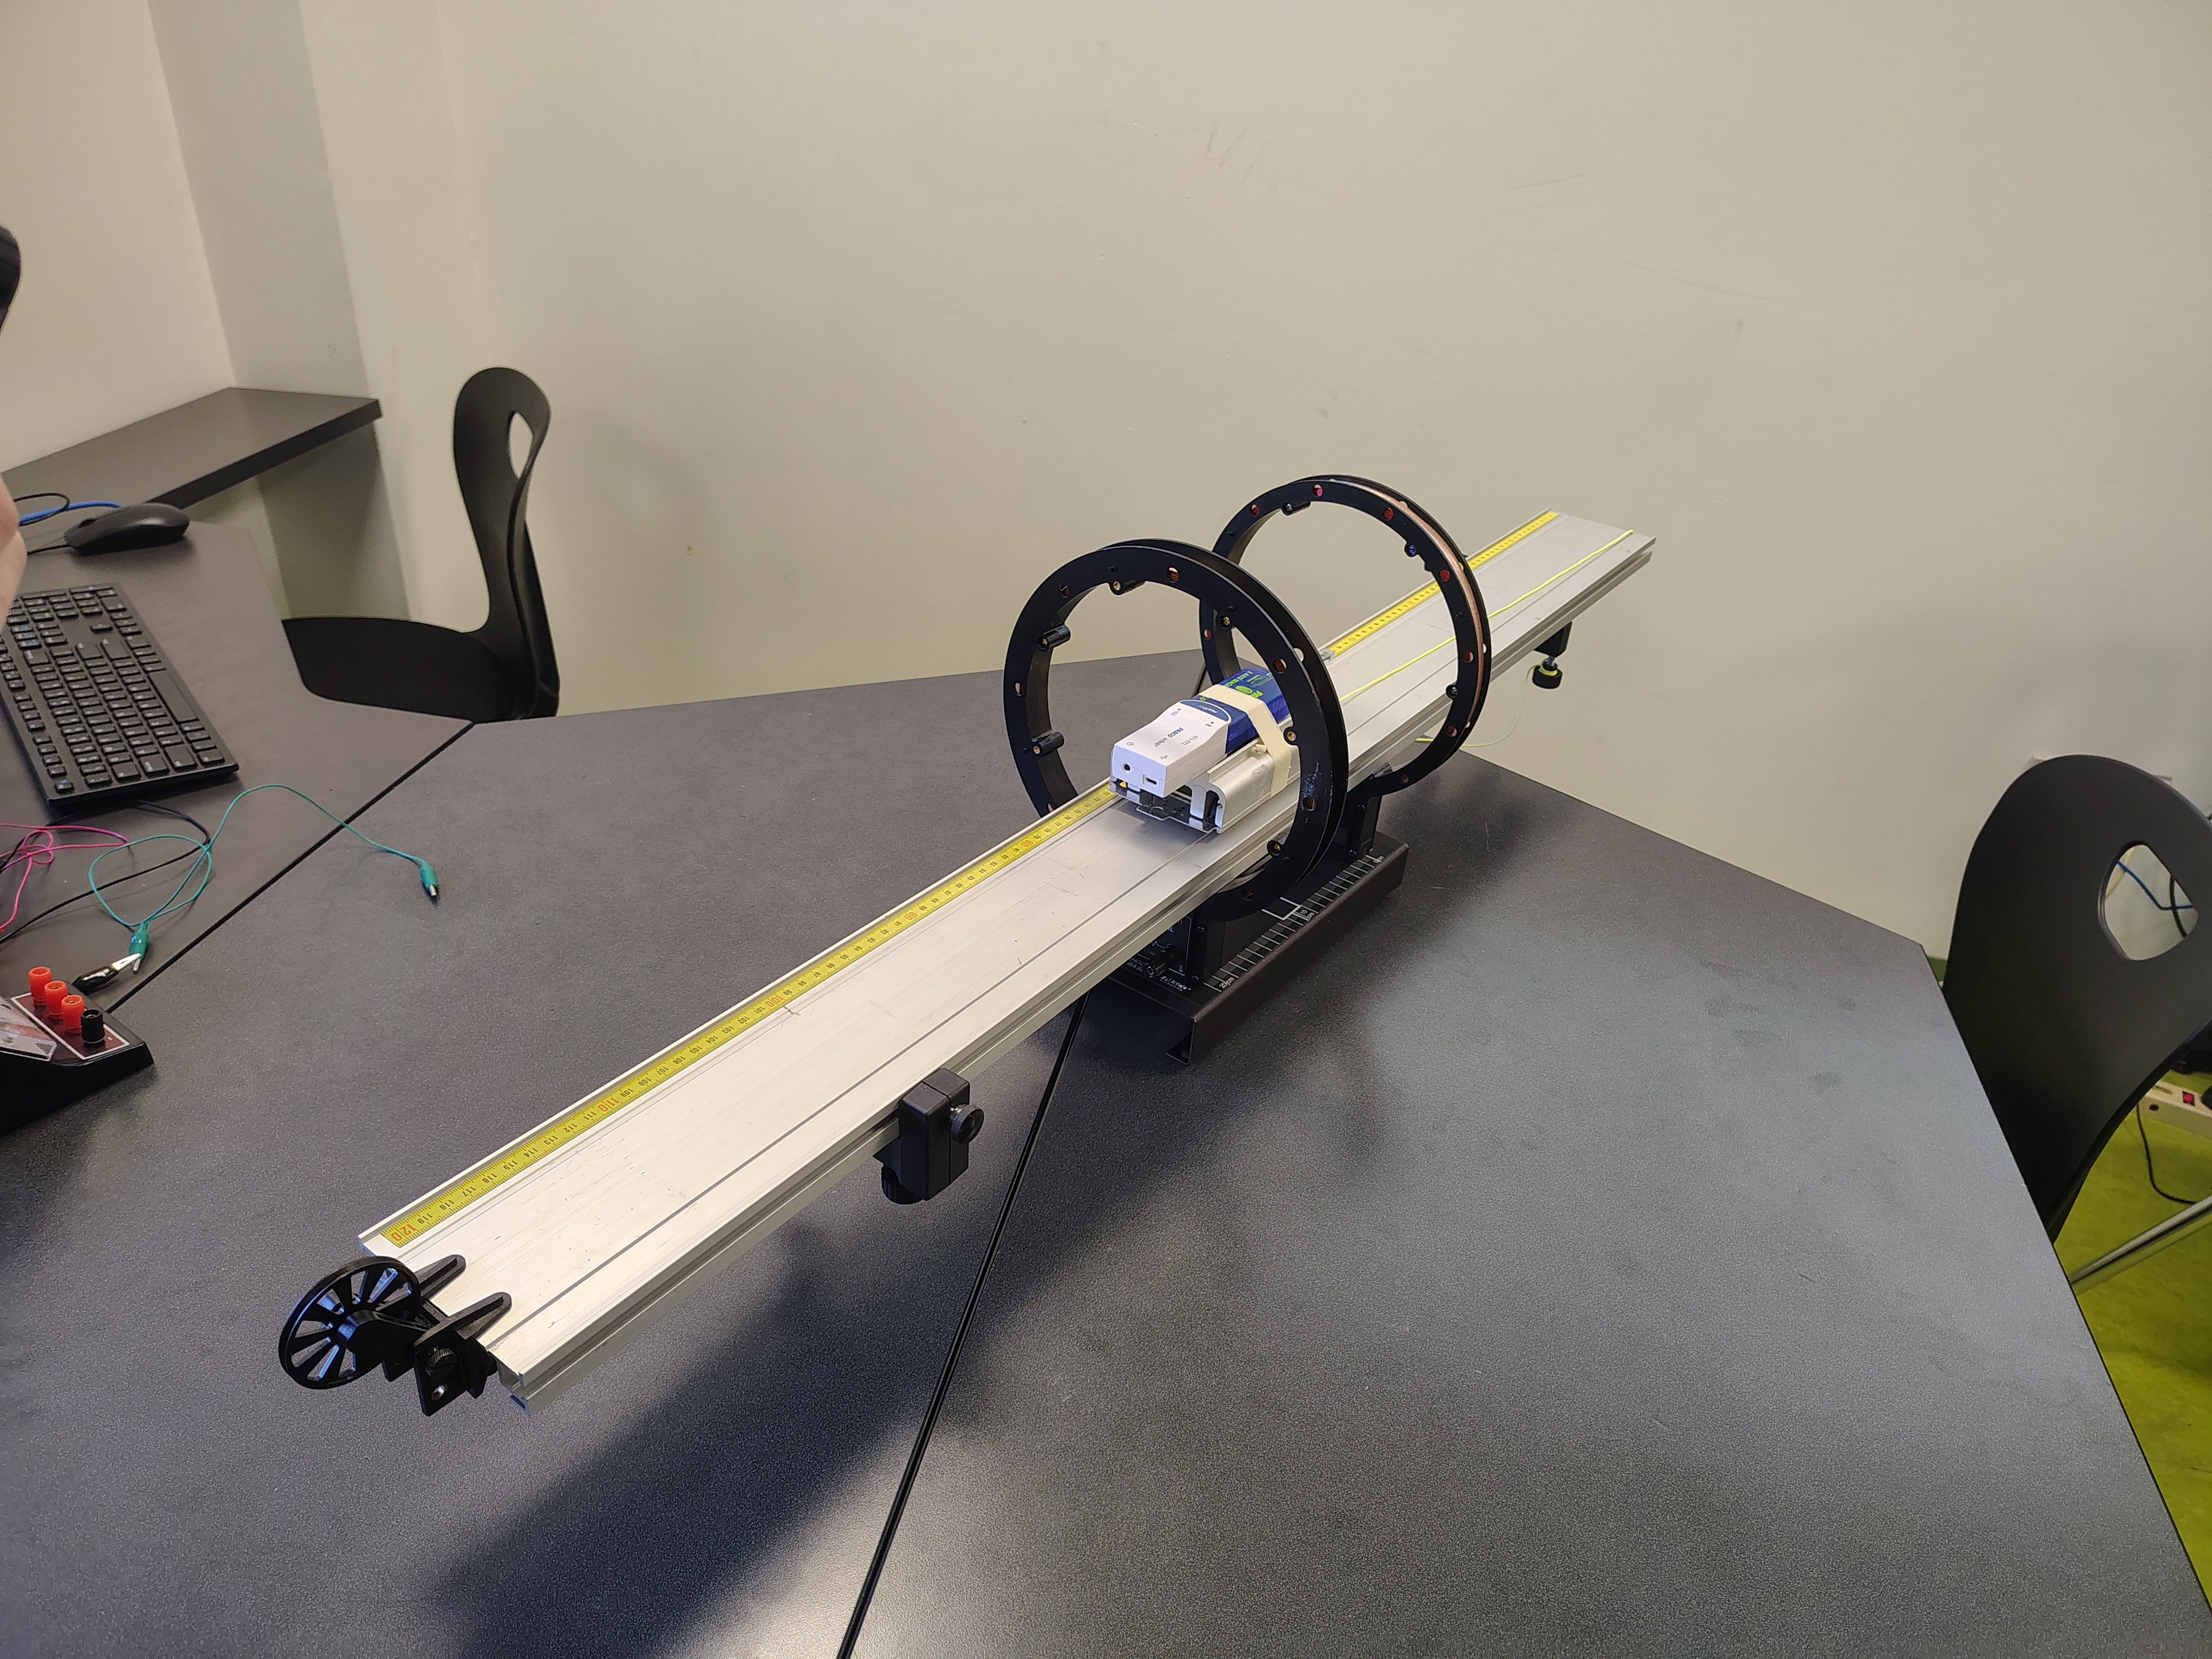
\includegraphics[width=0.5\linewidth]{figures/cart_and_rail.jpg}
    \caption{Pasco PS-2162 and Airlink setup on a cart on the rail with a 200 turn coil centered at $x=\SI{60 \pm 0.2}{\centi\metre}$}
    \label{fig: Cart and rail}
\end{figure}

\begin{figure}
    \centering
    \includegraphics[width=0.5\linewidth]{figures/full_setup.jpg}
    \caption{Complete experimental setup. Power source on the left set to \SI{3.5}{\volt} and ammeter between the source and the rail.}
    \label{fig: Full setup}
\end{figure}

\subsection{Data}
We calculated the average measured magnetic field over intervals of 5 seconds. Any intervals that were longer than \SI{5}{s} were truncated to keep the data collection intervals consistent across all data points. Additionally, run \#10 of the background dataset was not used for the data analysis due to it being shorter than \SI{5}{\second}. The difference between the background and coil runs was calculated to find the magnetic field generated by the coil itself. We found that all measurements were within \SI{50.4}{\micro\tesla} of the expected values. All raw data can be found in the appendix and references\footnote{All data can be found \href{https://github.com/LudioRex/E-M_coil_lab}{here}.\\(https://github.com/LudioRex/E-M\_coil\_lab)}

\begin{table}[H]
\vspace{4mm}
\begin{tabular}{|c|c|c|}
\hline
\multirow{2}{*}{Postition (cm $\pm0.2$)} & Magnetic field     & Magnetic field     \\ 
       &            strength (G $\pm0.01$)   & strength (T $\pm 1$E-06)\\ \hline 
30     & 3.33E-01 & 3.33E-05 \\
35     & 2.55E-01 & 2.55E-05 \\
40     & 2.92E-01 & 2.92E-05 \\
45     & 6.29E-01 & 6.29E-05 \\
50     & 1.39E+00 & 1.39E-04 \\
55     & 3.20E+00 & 3.20E-04 \\
60     & 4.64E+00 & 4.64E-04 \\
65     & 3.48E+00 & 3.48E-04 \\
70     & 1.76E+00 & 1.76E-04 \\
75     & 7.20E-01 & 7.20E-05 \\
80     & 5.52E-01 & 5.52E-05 \\
85     & 4.72E-01 & 4.72E-05 \\
90     & 2.58E-01 & 2.58E-05 \\ \hline
\end{tabular}
\caption{Average magnetic field strength due to the current carrying coil at different positions along the coil's axis. Calculated by taking the difference between the measured background and the measured magnetic field with current flowing through the coil.}
\label{table: Averages}
\end{table}

\begin{table}[H]
\begin{tabular}{|c|c|c|}
\hline
\multirow{2}{*}{Postition (cm $\pm0.2$)} & Axial magnetic  & Relative \\
& field strength (T) & uncertainty (\%) \\ \hline
30 & 1.44E-05 & 44\% \\
35 & 2.32E-05 & 50\% \\
40 & 4.02E-05 & 57\% \\
45 & 7.58E-05 & 65\% \\
50 & 1.54E-04 & 70\% \\
55 & 3.02E-04 & 59\% \\
60 & 4.14E-04 & 15\% \\
65 & 3.02E-04 & 59\% \\
70 & 1.54E-04 & 70\% \\
75 & 7.58E-05 & 65\% \\
80 & 4.02E-05 & 57\% \\
85 & 2.32E-05 & 50\% \\
90 & 1.44E-05 & 44\% \\ \hline
\end{tabular}
\caption{Calculated expected values of magnetic field strength at different positions along the coil's axis.}
\label{table: Theoretical}
\end{table}

\pagebreak
\subsection{Calculations}
\begin{center}
    Note that the sample calculations may contain slight discrepancies with the data due to rounding errors.
\end{center}

\begin{center}
    \textbf{Sample Calculations for the distance from center}
\end{center}
\begin{align*}
    z&=\SI{0.60 \pm 0.02}{\metre}-\SI{0.30\pm0.02}{\metre}\\
    &=\SI{0.30 \pm 0.04}{\metre}
\end{align*}

\vspace{2mm}
\begin{center}
    \textbf{Sample calculations for the expected magnetic field strength}
\end{center}

\begin{align*}
    {B}_{\substack{\text{coil} \\ \text{on-axis}}} &= N\frac{\mu_0IR^2}{2(z^2+R^2)^{3/2}} \\
    &=\frac{200\cdot\SI{4\pi e-7}{\tesla\metre\per\ampere}}{2}\\
    &\times\frac{\SI{0.34 \pm 0.01}{\ampere}\cdot\left(\frac{\SI{0.207 \pm 0.05}{\metre}}{2}\right)}{\left((\SI{0.30 \pm 0.04}{\metre})^2+\left(\frac{\SI{0.207 \pm 0.05}{\metre}}{2}\right)\right)^{3/2}}\\
    &=\SI{1.26e-4}{\tesla\metre\per\ampere}\\
    &\times\frac{(\SI{0.34}{\ampere}\pm2.94\%)\cdot\left(\frac{\SI{0.207}{\metre}\pm2.42\%}{2}\right)^2}{\left((\SI{0.30}{\metre}\pm13.3\%)^2+\left(\frac{\SI{0.207}{\metre}\pm2.42\%}{2}\right)\right)^{3/2}}\\
    &=\SI{1.26e-4}{\tesla\metre\per\ampere}\\
    &\times\frac{(\SI{0.34}{\ampere}\pm2.94\%)\cdot(\SI{0.1035}{\metre}\pm2.42\%)^2}{\left((\SI{0.30}{\metre}\pm13.3\%)^2+(\SI{0.1035}{\metre}\pm2.42\%)^2\right)^{3/2}}\\
    &=\SI{1.26e-4}{\tesla\metre\per\ampere}\\
    &\times\frac{(\SI{0.34}{\ampere}\pm2.94\%)\cdot(\SI{0.0107}{\metre\squared}\pm4.84\%)}{((\SI{0.09}{\metre\squared}\pm26.6\%)+(\SI{0.0107}{\metre\squared}\pm4.84\%))^{3/2}}\\
    &=\SI{1.26e-4}{\tesla\metre\per\ampere}\\
    &\times\frac{\SI{3.64e-3}{\ampere\metre\squared}\pm7.78\%}{(\SI{0.09 \pm 0.02}{\metre\squared}+\SI{0.0170 \pm 0.0005}{\metre\squared})^{3/2}}\\
    &=\SI{1.26e-4}{\tesla\metre\per\ampere}\\
    &\times\frac{\SI{3.64e-3}{\ampere\metre\squared}\pm7.78\%}{(\SI{0.1071 \pm 0.0205}{\metre\squared})^{3/2}}\\
    &=\SI{1.26e-4}{\tesla\metre\per\ampere}\times\frac{\SI{3.64e-3}{\ampere\metre\squared}\pm7.78\%}{(\SI{0.1071}{\metre\squared}\pm19.2\%)^{3/2}}\\
    &=\SI{1.26e-4}{\tesla\metre\per\ampere}\times\frac{\SI{3.64e-3}{\ampere\metre\squared}\pm7.78\%}{\SI{0.035}{\cubic\metre}\pm28.8\%}\\
    &=\SI{1.26e-4}{\tesla\metre\per\ampere}\times(\SI{0.104}{\ampere\per\metre}\pm36.6\%)\\
    &=\SI{1.31e-5}{\tesla}\pm36.6\%\\
   % &=(1.3\times10^{-5}\pm5\times10^{-6})\,\text{T}
   &=\SI{13 \pm 5}{\micro\tesla}
\end{align*}

\begin{figure}[H]
    \centering
    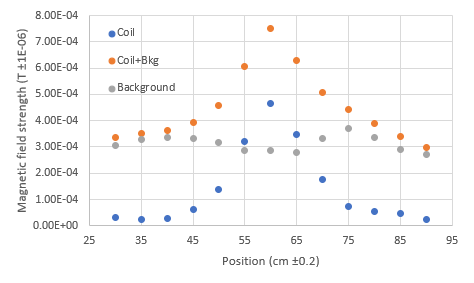
\includegraphics[width = \linewidth]{figures/sets_graph_zoomed.png}
    \caption{Comparison of the two different measured data sets, background and coil+bkg, and the calculated coil magnetic field at different positions along the coil's axis.}
    \label{fig: Sets graph}
\end{figure}

\begin{figure}[H]
    \centering
    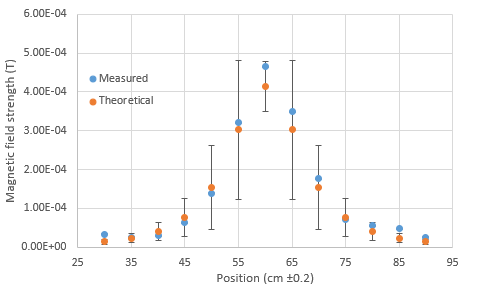
\includegraphics[width = \linewidth]{figures/measured_vs_theoretical_revised_zoomed.png}
    \caption{Measured magnetic field strength along the coil's axis compared to the expected values. Error bars represent uncertainty.}
    \label{fig: Measured vs theoretical}
\end{figure}

\begin{figure}[H]    \centering
    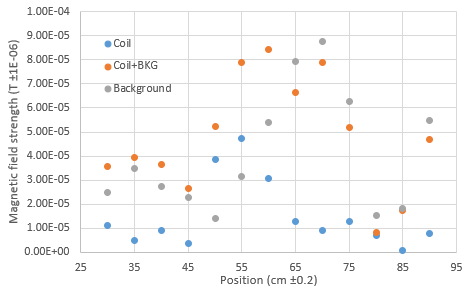
\includegraphics[width = \linewidth]{figures/perpendicular_sets_graph_revised.png}
    \caption{Comparison of the two different measured data sets, background and coil+bkg, and the calculated coil magnetic field perpendicular to the coil's axis at different positions along said axis.}
    \label{fig: Perpendicular sets graph}
\end{figure}

\vspace{1cm}
\subsection{Results}
Figure \ref{fig: Measured vs theoretical} shows the difference between the values we measured and those predicted by our model. Three of the points in this graph are outside the uncertainty range of the expected values, those being the points at $x\in\{\SI{30 \pm 0.2}{\centi\metre};\, \SI{85 \pm 0.2}{\centi\metre};\, \SI{90 \pm 0.2}{\centi\metre}\}$. These points were outside the range by \SI{12.5}{\micro\tesla}, \SI{12.4}{\micro\tesla}, and \SI{5.08}{\micro\tesla} respectively.

\section{Discussion}
Our results are very close to those predicted by the model. It is important to note that the discrepant points are at the edge of the measured range, and we can also see from figure \ref{fig: Sets graph} that they do not follow the trend of the other points, being higher than the previous point in a descending function. Furthermore, these points are outside the uncertainty range by only small amounts, which, all things considered, is why we believe that despite these discrepancies with the model we can still consider that our results support the theoretical basis for this experiment.

We must also note that, even though we did our best to center the rail along the axis of the coil, we were clearly off center given that our data shows that there was some magnetic field strength perpendicular to the axis where we were taking our measurements, which would not be expected if we really were on the axis. Additionally, we must also mention that it did not occur to us, at the time of the experiment, to align the rail vertically which would also affect our results.

Additionally, any change in the background field, due, for example, to the use of nearby electronic devices, would also significantly influence the results obtained.

The number of data points also limits our ability to draw meaningful conclusions, it would have been interesting to take measurements at more positions to be able to draw stronger conclusions.

Moving forward, now that we have established a predictable magnetic field, it would be interesting to study magnetic flux and possibly induction. Since we can predict the change in magnetic flux experienced by an object with a known velocity, we could experiment with inductions, which could help validate our model on this subject.

\section{Conclusion}
Our results support the validity of our current electromagnetic model, since most of our data points match the expected values. In fact, the largest difference between the theoretical and expected values was \SI{50.4}{\micro\tesla} and for the values outside of the uncertainty range, the furthest was only \SI{12.5}{\micro\tesla} from being within the uncertainty. The results of this experiment weren't particularly impressive, as plenty of electronic devices rely on this model of electromagnetism to function. Nonetheless, it is important to stay on the lookout for any discrepancies that might reveal a flawed understanding of electromagnetism, as it might lead to new innovation and to overall safer electronic devices.

\section{Acknowledgments}
\begin{center}
    This experiment was conducted in collaboration with Evan Parasol, Alex Xia, and Andy Yu.
\end{center}

\clearpage
\section{Appendices}
\begin{table}[H]
\centering
\begin{tabular}{|c|c|c|c|}
\hline
Run \# & Position (cm) & B (G $\pm$0.01) & B (T$\pm$1E-06) \\ \hline
1 & 30 & 3.04E+00 & 3.04E-04 \\
2 & 35 & 3.27E+00 & 3.27E-04 \\
3 & 40 & 3.34E+00 & 3.34E-04 \\
4 & 45 & 3.31E+00 & 3.31E-04 \\
5 & 50 & 3.17E+00 & 3.17E-04 \\
6 & 55 & 2.87E+00 & 2.87E-04 \\
7 & 60 & 2.85E+00 & 2.85E-04 \\
8 & 65 & 2.79E+00 & 2.79E-04 \\
9 & 70 & 3.32E+00 & 3.32E-04 \\
10 & 75 & 3.62E+00 & 3.62E-04 \\
11 & 75 & 3.70E+00 & 3.70E-04 \\
12 & 80 & 3.35E+00 & 3.35E-04 \\
13 & 85 & 2.91E+00 & 2.91E-04 \\
14 & 90 & 2.70E+00 & 2.70E-04 \\ \hline
\end{tabular}
\caption{Average background magnetic field strength(B) measured at different positions along the coil's axis.}
\end{table}

\begin{table}[H]
\centering
\begin{tabular}{|c|c|c|c|}
\hline
Run \# & Position (cm) & B (G $\pm$0.01) & B (T$\pm$1E-06) \\ \hline
1 & 30 & 3.37E+00 & 3.37E-04 \\
2 & 35 & 3.53E+00 & 3.53E-04 \\
3 & 40 & 3.63E+00 & 3.63E-04 \\
4 & 45 & 3.94E+00 & 3.94E-04 \\
5 & 50 & 4.56E+00 & 4.56E-04 \\
6 & 55 & 6.07E+00 & 6.07E-04 \\
7 & 60 & 7.49E+00 & 7.49E-04 \\
8 & 65 & 6.28E+00 & 6.28E-04 \\
9 & 70 & 5.08E+00 & 5.08E-04 \\
10 & 75 & 4.42E+00 & 4.42E-04 \\
11 & 80 & 3.91E+00 & 3.91E-04 \\
12 & 85 & 3.38E+00 & 3.38E-04 \\
13 & 90 & 2.96E+00 & 2.96E-04 \\ \hline
\end{tabular}
\caption{Average magnetic field strength (B), measured with a \SI{0.34 \pm 0.01}{\ampere} current flowing thought the coil, at different positions along the coil's axis.}
\end{table}

\begin{figure}[H]
    \centering
    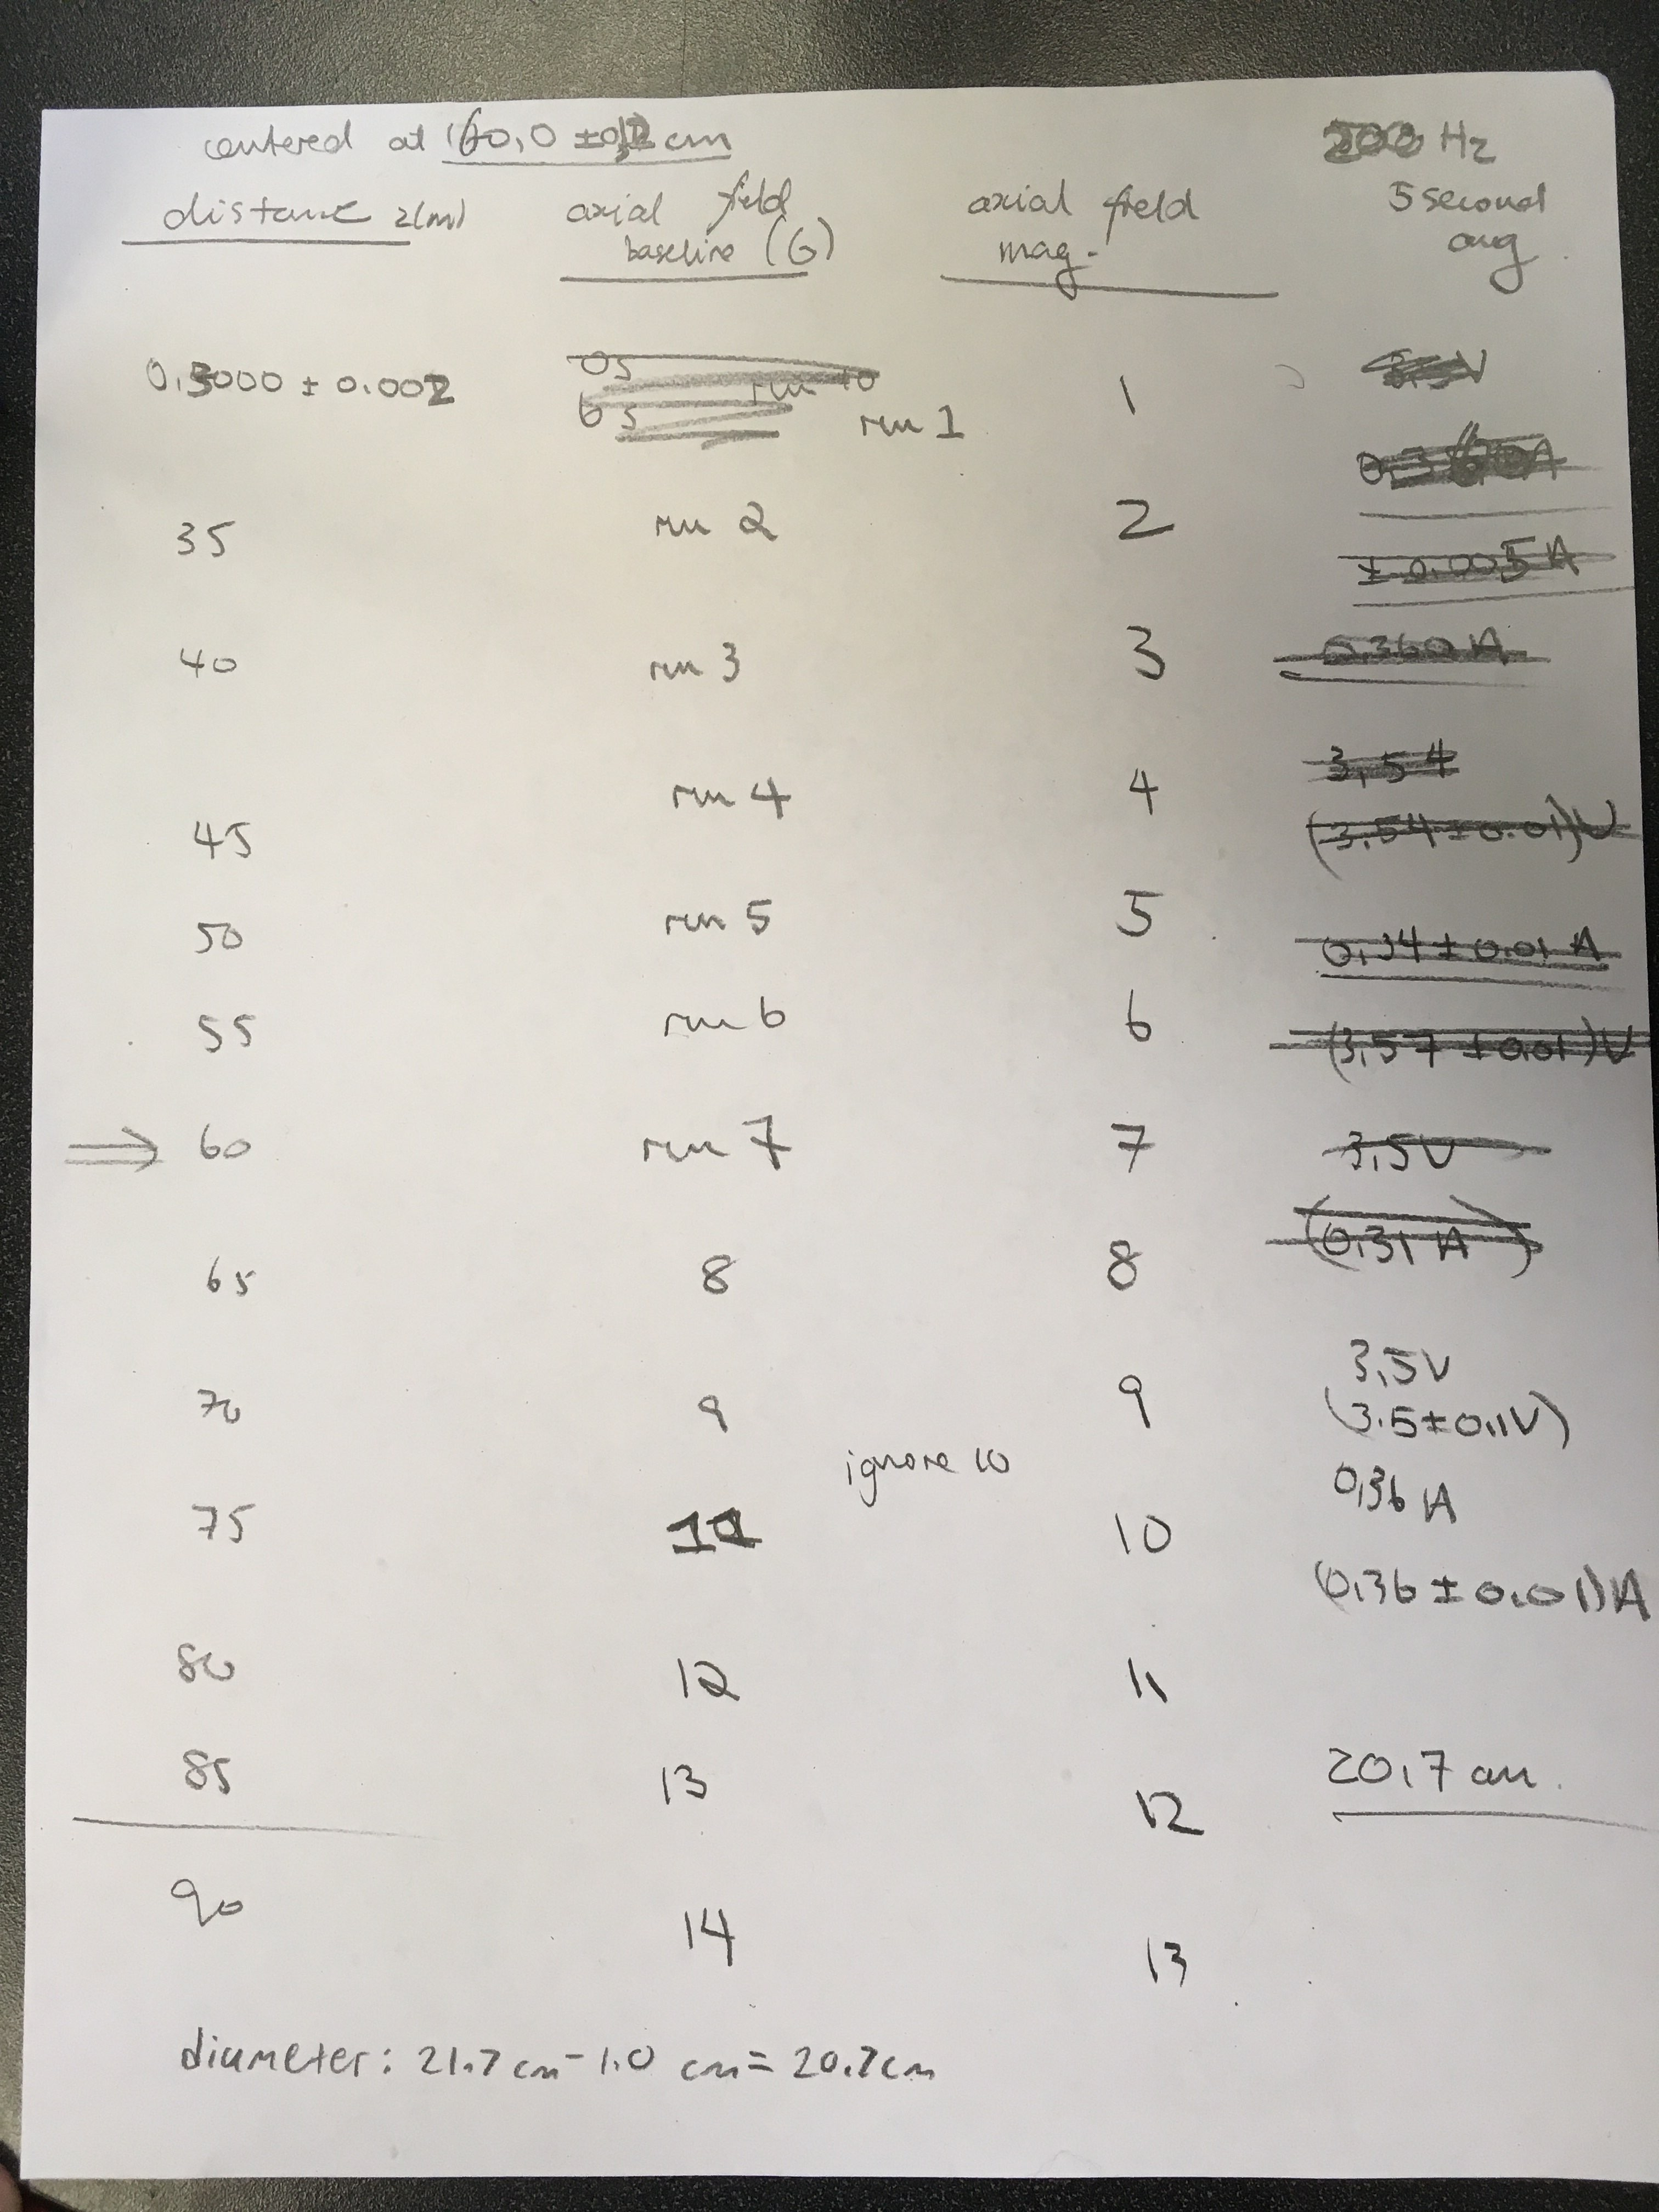
\includegraphics[width=0.5\linewidth]{figures/data_sheet.jpg}
    \caption{Raw data sheet used during the experiment to note the properties of the coil and of each run.}
\end{figure}


\end{document}
